%-------------------------------------------------
%	Version: 0.0
%	fecha de entrega
%
%-------------------------------------------------

\documentclass[11pt]{report}

%packages
\usepackage{graphicx}
\usepackage{subcaption}

\usepackage[utf8]{inputenc}
\usepackage[spanish, es-nodecimaldot]{babel}
\usepackage{setspace}
\usepackage{ragged2e}

\usepackage{amsmath}
\usepackage{amsthm}
\usepackage{amssymb}
\usepackage{mathtools}
\usepackage{siunitx}
\usepackage[thinc]{esdiff} %derivadas faciles
\usepackage{physics} %algunos simbolos de derivadas

%path donde se encuentran las imagenes
\graphicspath{ {./figuras/} }

%---------------------------------------------------------------
%ABREVIACIONES DE COMANDOS

\theoremstyle{plain}
\newtheorem{thm}{Teorema}[chapter] % reset theorem numbering for each chapter

\theoremstyle{definition}
\newtheorem{defn}[thm]{Definición} % definition numbers are dependent on theorem numbers
\newtheorem{exmp}[thm]{Ejemplo} % same for example numbers

\newcommand{\chaptercontent}{
\section{Basics}
\begin{defn}Here is a new definition.\end{defn}
\begin{thm}Here is a new theorem.\end{thm}
\begin{thm}Here is a new theorem.\end{thm}
\begin{exmp}Here is a good example.\end{exmp}
\subsection{Some tips}
\begin{defn}Here is a new definition.\end{defn}
\section{Advanced stuff}
\begin{defn}Here is a new definition.\end{defn}
\subsection{Warnings}
\begin{defn}Here is a new definition.\end{defn}
}

\usepackage{biblatex}
%\addbibresource{Tarea1.bib}

\begin{document}

\begin{titlepage}
\title{Tarea2}

%-------------------------------------------------
%PORTADA
%-------------------------------------------------

	\centering
	{\scshape\LARGE Universidad Autónoma de Yucatán  \\ Facultad de ingeniería\par}
	\vspace{1cm}
	{\scshape\Large Introducción al Caos\par}
	\vspace{1.5cm}
	{\huge\bfseries Tarea2\par}
	\vspace{0.7cm}
	{\begin{figure}[!h]
	\centering
    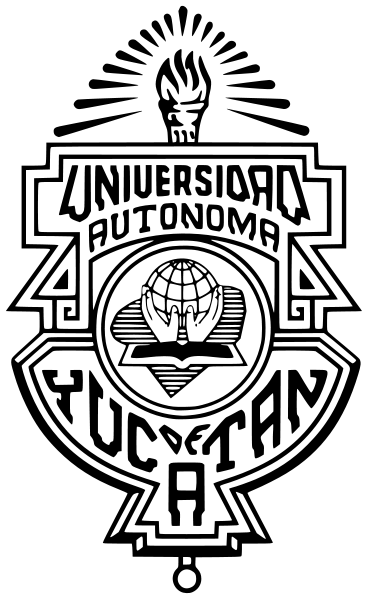
\includegraphics[scale=0.3]{UADY.png}
	\end{figure}}
	\vspace{0.7cm}
	{\Large\itshape Erick Al. Casanova Cortés\par}
	{\Large\itshape Matricula: 15014866\par}
	\vfill
	{\scshape\Large Docente\par
	Dr. César Acosta\par}
	\vfill
	{\Large{\bfseries Fecha de entrega: Febrero 8, 2021} }

	\vfill
	
\end{titlepage}

%-------------------------------------------------
%Inicio del documento
%-------------------------------------------------

%--- primer ejercicio
\textit{Utilice el análisis gráfico para describir en cada función las posiciones de los puntos fijos, establecer un rango de trabajo, encontrar (si existen) los puntos de silla de montar, así como algunos puntos posteriores donde se observe bifurcación. Encuentre las funciones de la segunda, tercera y cuarta iteración y para estas halle los puntos periódicos, en donde utilizando el criterio de la derivada de la primera iteración diga si son de atracción o de repulsión, verifique sus resultados con la evaluación de la derivada de la propia iteración.}

$f(x) = x^3 + c$

$f(x) = cx^2 + x$

$f(x) = x^3 + cx^2 + x$

$f(x) = c\sin(x)$

%--- segundo ejercicio
\textit{Dada la función $f (x) = x^3 + c$, halle la función de la cuarta iteración, encuentre los puntos
periódicos para esta ecuación, tomando una secuencia de periodicidad 4 y utilizando las bases 2 y 3 describa en que iteración se encuentra cada dígito de esa serie 4-periódico, utilizando al menos 5 dígitos de precisión.}

%--- tercer ejercicio
\textit{Dada la función $f (x) = c \sin(x) $, halle la función de la séptima iteración, encuentre los puntos periódicos para esta ecuación, tomando una secuencia de periodicidad 7 y utilizando las bases 2 y 3 describa en que iteración se encuentra cada dígito de esa serie 7-periódico, utilizando al menos 5 dígitos de precisión}

%--- cuarto ejercicio
\textit{Dada la función $f(x) = x^3 + cx^2 + x$, halle la función de la décima iteración y tome una secuencia de números periódicos cualquiera y utilizando las bases 2 y 3 describa en que iteración se encuentra cada dígito de esa serie n-periódico, utilizando al menos 5 dígitos de precisión}

%--- quinto ejercicio
\textit{Sea $f (x) = x^3 + c$, tome algunos (4) números cualesquiera como semilla halle la suerte de esta en la centésima iteración y verifique si alguno se volvió periódico y utilizando las bases 2 y 3 describa en que iteración se encuentra cada dígito elegido, utilizando al menos 5 dígitos de precisión}

%--- sexto ejercicio
\textit{Utilizando la expansión ternaria (utilice series), encuentre los números racionales que corresponda}


0.212121...\\
0.022022022...\\
0.00222...\\
0.212010101...\\
0.0101101101...\\
%-------------------------------------------------
%Final del documento
%-------------------------------------------------

\end{document}
